\documentclass[../main.tex]{subfiles}

\lstMakeShortInline[columns=fixed, basicstyle=\bfseries]|

\begin{document}
Im Gegensatz zu General Purpose CPUs lassen sich mithilfe von Coprozessoren deutlich höhere Parallelisierungsgrade erzielen. Gegenüber GPUs haben sie den Vorteil, dass die Kerne eines Coprozessors einen größeren Befehlssatz verfügen, mit dem sie nicht nur Befehlssequenzen, sondern auch bedingte Sprünge ausführen können. Mit GPUs lässt sich dagegen eine weitaus höhere Parallelität erreichen. Mit der Max Pooling-Operation ist die Fähigkeit von Coprozessoren, auch Code mit Verzweigungen parallel auszuführen, von Nutzen. 

In dieser Arbeit soll auch eine Implementierung des CNNs erstellt werden, die Berechnungen an Coprozessoren. Ein direkter Vergleich dieser Implementierung mit Tensorflow hat nur bedingte Aussagekraft, da Tensorflow laut der offiziellen Dokumentation nur für den Einsatz auf CPUs, GPUs und TPUs optimiert ist. Coprozessoren werden von Tensorflow dagegen nicht explizit unterstützt. (vgl. \cite{aboutTensorflow}) Ein Vergleich zwischen dieser Implementierung und den anderen beiden in dieser Arbeit behandelten optimierten Implementierungen lässt allerdings Rückschlüsse darauf ziehen, wie der Performancegewinn unter Zuhilfenahme eines Coprozessors einzuordnen ist. 

Die DHBW Stuttgart besitzt einen Server, der mit einer General Purpose CPU(Intel Xeon E5-2650L) und zwei Coprozessoren(Intel Xeon Phi) ausgestattet ist. Beim Xeon Phi handelt es sich um eine PCIe-Erweiterungskarte, auf der eine spezielle CPU mit 60 Kernen und einer Taktrate von 1\,GHz, sowie ein DDR5-Arbeitsspeicher mit einer Größe von 8\,GB verbaut sind. Für diese Arbeit wurde den Studenten freundlicherweise ein SSH-Zugang zur Verfügung gestellt. Die in diesem Kapitel betrachtete Implementierung soll auf dem genannten Server getestet und dementsprechend auch für dessen Prozessoren optimiert werden. 

\section{Intel Xeon Phi Coprozessor}
Beim Intel Xeon Phi handelt es sich um einen Coprozessor, der in Form einer PCIe-Erweiterungskarte (siehe Abbildung \ref{pic:xeonphicard}) mit dem Hostsystem verbunden werden kann und numerische Operationen durch Parallelisierung über bis zu 72 Rechenkerne, sowie durch Vektorisierung unterstützt. Zusätzlich zum Prozessor selbst ist auf der Erweiterungskarte ein DDR5-Arbeitsspeicher verbaut. Bei Bedarf kann der Xeon Phi ein eigenes Betriebssystem ausführen und damit Programme komplett unabhängig vom Hostsystem abarbeiten. (vgl. \cite{intelxeonphiprocessors})
\begin{figure}
    \centering 
       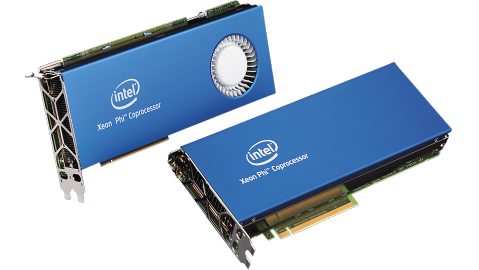
\includegraphics[width=0.5\textwidth]{../images/Schmidt/xeon_phi_cards.png} 
    \caption {Eine Erweiterungskarte mit einem Intel Xeon Phi (Quelle: \parencite{intelMICarchitecture})} 
    \label{pic:xeonphicard} 
\end{figure} 

\subsection{Geschichte}
%TODO

\subsection{MIC-Archtektur}
Der Xeon Phi basiert auf der von Intel entwickelten MIC-Architektur. MIC steht dabei für "Many Integrated Cores". 
Wie in Abbildung \ref{pic:knightscorner} am Beispiel der Mikroarchitektur Knigths Corner zu sehen ist, kommunizieren die Kerne, der Arbeitsspeicher und die PCIe-Schnittstelle untereinander über einen Ringförmigen Datenbus mit einer Busbreite von 64 Bytes. (vgl. \cite{xeonphiJumpstart})
\begin{figure}
    \centering 
       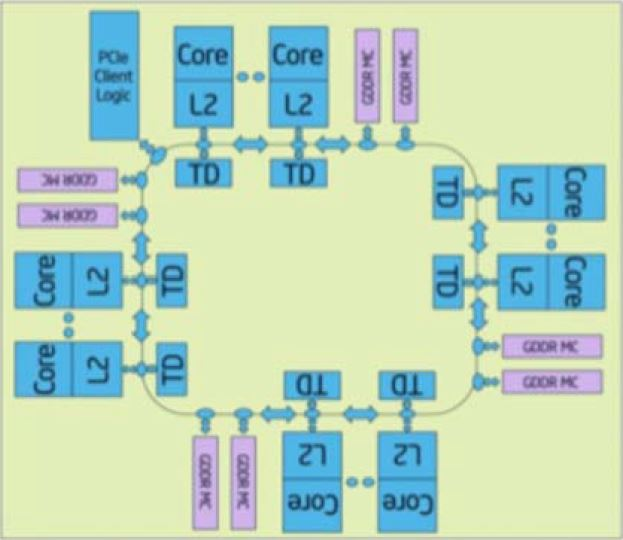
\includegraphics[width=0.5\textwidth]{../images/Schmidt/intel_mic_diagram.jpg} 
    \caption {Mikroarchitektur Knights Corner (Quelle: \parencite{xeonphiJumpstart})}
    \label{pic:knightscorner} 
\end{figure}
Zur Verminderung der Verlustleistung und der damit verbundenen Abwärme takten die einzelnen Rechenkerne langsamer als vergleichbare General Purpose CPUs. Der hohe Durchsatz des Coprozessors kann erreicht werden, weil Operationen auf viele Kerne verteilt und Operanden mithilfe der breiten Speicheranbindung zeitnah abgerufen werden können. (vgl. \cite{xeonphiJumpstart})

\subsection{Anbindung an das Hostsystem}
Mit dem Hostsystem ist der Xeon Phi über PCIe x16 verbunden. Dieser Bus lässt eine Bandbreite von 8\,GB/s zu. Verglichen mit der Bandbreite der Speicheranbindung des Hostsystems, sowie des Datenbusses innerhalb des Xeon Phi ist diese Bandbreite sehr gering. Abbildung \ref{pic:xeonphiBandwidths} vermittelt einen Eindruck über die Busbreiten innerhalb eines Systems mit zwei Prozessoren, DDR3-Arbeitsspeichern, und einem Rechenbeschleuniger bestehend aus einem Intel Xeon Phi und DDR5-Speicher. (vgl. \cite{interDeviceCommunication})
\begin{figure}
    \centering 
       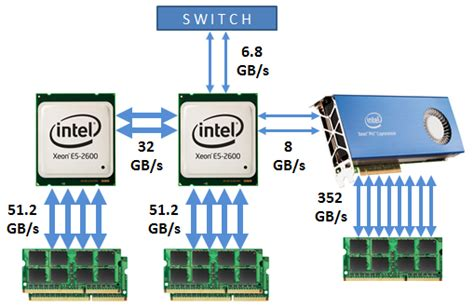
\includegraphics[width=0.5\textwidth]{../images/Schmidt/xeonphi_bandwidths.jpg} 
    \caption {Busbandbreiten eines Systems mit DDR3-Arbeitsspeicher und Intel Xeon Phi (Quelle: \parencite{interDeviceCommunication})}
    \label{pic:xeonphiBandwidths} 
\end{figure}
In Anwendungen, bei denen Daten zwischen dem Hostsystem und dem Xeon Phi geteilt werden müssen, ist die Übertragung dieser Daten eine kritischer Engpass. Der Aufwand zur Kommunikation zwischen den beiden Systemen hat großen Einfluss auf die Performance des Gesamtsystems. Der Programmierer hat dafür Sorge zu tragen, dass der Datenaustausch zwischen dem Host und dem Rechenbeschleuniger möglichst effizient verläuft. Die Beachtung folgender Faustregeln trägt zu einer hohen Effizienz des Offloads bei: 
\begin{itemize}
\item Daten zum Coprozessor transferieren und dort behalten (vgl. \cite{xeonphiJumpstart})
\item Möglichst große Rechenoperationen auslagern (vgl. \cite{xeonphiJumpstart})
\item Auf dem Coprozessor bereits existierende Daten wiederverwerten (vgl. \cite{xeonphiJumpstart})
\end{itemize}

\section{Nutzungsmodelle}
Zur Planung einer Software, die einen Xeon Phi benutzen soll, gehört die Überlegung, welche Operationen sich zur Ausführung auf dem Coprozessor eignen und welche Rechenschritte auf dem Hostsystem ausgeführt werden sollten. Abhängig von dieser Verteilung sollte bestimmt werden, auf welche Weise der Coprozessor verwendet werden soll. Es kann zwischen mehreren Nutzungsmodellen gewählt werden, die bekanntesten davon werden nachfolgend vorgestellt. 

\subsection{Automatic Offload}
Das für den Programmierer einfachste Nutzungsmodell ist Automatic Offload. Bei diesem Modell entscheidet das Programm zur Laufzeit, ob numerische Berechnungen auf dem Coprozessor oder dem Hostsystem ausgeführt werden sollen. Der Programmierer muss dazu keine Vorkehrungen im Quellcode treffen. Die dazu notwendige Entscheidungslogik ist bereits in einigen vorkompilierten Bibliotheken, wie der Math Kernel Library von Intel enthalten. Das bedeutet, dass sich der Programmierer bei der Nutzung von Funktionen dieser Bibliotheken keine Gedanken darüber machen muss, wann eine Auslagerung an den Coprozessor sinnvoll ist oder wie diese veranlasst wird. Ein Nachteil dieses Modells besteht allerdings darin, dass es sich nur auf dafür geeignete Bibliotheksfunktionen anwenden lässt. Zur Auslagerung von eigenem Anwendungscode lässt sich dieses Modell nicht anwenden. 

\subsection{Compiler-Assisted Offload} \label{phiCompAssistOffload}
Für den Fall, dass aufwändige Abschnitte des Anwendungscodes auf den Coprozessor ausgelagert werden sollen, kann dies dem Compiler explizit mitgeteilt werden. In C/C++ lässt sich dies mithilfe des Pragmas |#pragma offload| bewerkstelligen. (vgl. \cite{xeonphiQuickstart}) Das nachfolgende Codebeispiel soll verdeutlichen, wie dieses Pragma anzuwenden ist. 
\begin{lstlisting}[language=c, caption={Beispiel für eine Funktion, die ausgelagert werden soll (Quelle: \parencite{xeonphiQuickstart})} , captionpos=b, label=lst:compoffloadBefore, frame=single, linewidth=\textwidth, breaklines=true]
float reduction(float *data, int size) 
{ 
	float ret = 0.f; 
	for (int i=0; i<size; ++i) 
	{
		ret += data[i]; 
	} 
	return ret; 
}
\end{lstlisting}
\begin{lstlisting}[language=c, caption={Beispielfunktion mit pragma zur Auslagerung(Quelle: \parencite{xeonphiQuickstart})}, captionpos=b, label=lst:compoffloadAfter, frame=single, linewidth=\textwidth, breaklines=true]
float reduction(float *data, int size) 
{ 
	float ret = 0.f; 
	#pragma offload target(mic) in(data:length(size))
	for (int i=0; i<size; ++i) 
	{
		ret += data[i]; 
	} 
	return ret; 
}
\end{lstlisting}
Wie in den obigen Beispielen zu sehen ist, genügt bereits das Hinzufügen einer Zeile zum Quellcode, um einen zusammenhängenden Codeabschnitt (in diesem Beispiel die |for|-Schleife) an den Coprozessor auszulagern. Die Angabe |target(mic)| legt dabei fest, dass an einen Coprozessor mit der MIC-Architectur ausgelagert werden soll. Die Angabe |in(data:length(size))| teilt dem Compiler mit, dass das Array |data| mit der Größe |size| zum Coprozessor übertragen hin, aber nicht mehr zurück übertragen werden muss. Für die Variable |ret| gibt es keine explizite Angabe, daher wird sie per Default vor der Berechnung zum Coprozessor hin und anschließend zum Hostsystem zurück übertragen. (vgl. \cite{xeonphiQuickstart})

Auch wenn dieses Pragma im Quellcode angegeben ist, gibt es keine Garantie dafür, dass der betroffene Codeabschnitt tatsächlich vom Coprozessor bearbeitet wird. Laut dem C99-Standard ist es dem Compiler überlassen, wie Pragmas in einem C-Programm zu behandeln sind. Pragmas sind sogar explizit dafür vorgesehen, compilerspezifische Features zu steuern. Wenn das Programm mit einem Compiler übersetzt wird, der nicht für den Offload auf einen Xeon Phi vorgesehen ist, dann sollte er dieses Pragma ignorieren und bestenfalls mit einer Warnung auf das unbekannte Pragma hinweisen. (vgl. \cite{gccDokuPragmas}) Selbst wenn der Compiler Offload-Code für einen Xeon-Phi erzeugt, dann muss das noch nicht zwangsläufig heißen, dass der Offload tatsächlich durchgeführt wird. Wenn der Coprozessor zur Laufzeit nicht Verfügbar ist, dann wird der auszulagernde Codeabschnitt trotzdem auf dem Hostsystem ausgeführt. (vgl. \cite{xeonphiQuickstart})

Compiler Assisted Offload ist dann hilfreich, wenn Teile des Anwendungscodes auf den Coprozessor ausgelagert werden sollen. Es liegt jedoch in der Verantwortung des Programmierers, geeignete Codeabschnitte auszuwählen und die zu übertragende Datenmenge gering zu halten. 

\subsection{Native}
Eine dritte Möglichkeit besteht darin, Anwendungen nativ auf dem Coprozessor laufen zu lassen. Dazu muss die Anwendung mit unter Angabe einiger zusätzlicher Compileroptionen gebaut werden. Die dabei erstellte Binary ist dann auf dem Hostsystem selbst nicht lauffähig. Sie lässt sich allerdings auf den Xeon Phi übertragen. Dieser verfügt über ein auf dem Linux-Kernel basierendes Betriebssystem, auf dem die erzeugte Binary ausgeführt werden kann. Bei einer nativen Programmausführung muss nur einmalig die Binary zum Xeon Phi übertragen werden. Zur Laufzeit ist dann keine Kommunikation mit dem Hostsystem notwendig. Auf diese Weise kann der Flaschenhals zwischen den beiden Systemen umgangen werden. (vgl. \cite{xeonphiQuickstart})

Es ist allerdings nicht für jede Software von Vorteil, nativ auf dem Coprozessor zu laufen. Die Performance bei der Ausführung serieller Programmabschnitte nimmt bei diesem Nutzungsmodell deutlich ab, da der Xeon Phi für diese Aufgaben nicht optimiert ist. Die Performance bei der Ausführung von parallel berechenbaren Operationen nimmt nicht signifikant zu oder ab, denn sobald notwendigen alle Instruktionen und Operanden zur Verfügung stehen, wird die eigentliche Berechnung auf die gleiche Art ausgeführt. Was tatsächlich eingespart wird, sind die Datentransfers zwischen dem Hostsystem und dem Coprozessor. Aufgrund dieser Informationen kann eingeschätzt werden, ob sich eine native Programmausführung gegenüber einer Offload-Variante lohnt: Bei seltenen Wechseln zwischen längeren seriellen und parallelen Abschnitten sollte das Programm auf dem Hostsystem ausgeführt werden und bei Bedarf Rechenoperationen an den Xeon Phi auslagern. Wenn es erforderlich ist, das Programm in viele kurze serielle und parallele Abschnitte zu unterteilen, dann nimmt die Wahrscheinlichkeit zu, dass sich die native Ausführung der gesamten Anwendung auf dem Xeon Phi lohnt. (vgl. \cite{xeonphiQuickstart})

\section{Compiler}
Zum Übersetzen des in diesem Abschnitt zu erstellenden Programms kommt der Intel C++ Compiler zum Einsatz. Dieser wurde von Intel speziell zur Übersetzung und Optimierung von Code für Intels Prozessoren entwickelt, ist aber nicht auf diese Anwendungen beschränkt. Die erstellten Binaries sind auf allen Prozessoren ausführbar, die die Architekturen Intel64 oder IA-32 unterstützen. Darüber unterstützt der Compiler die Auslagerung von parallelisierbaren Rechenoperationen auf Intels Rechenbeschleuniger. Zu diesen gehören GPUs, die gemeinsam mit den eigentlichen CPUs in einigen Intel-Prozessoren enthalten sind, sowie Coprozessoren auf Basis der Intel MIC-Architektur, also auch der Xeon Phi. (vgl. \cite{iccDocumentation})

Zur Erzeugung eines Programms, das auf mehrere Prozessoren verschiedener Architekturen verteilt werden soll, muss der Compiler heterogene Programme erzeugen. Bei der Nutzung eines Xeon-Phi und eines Nutzungsmodells, das Offload verwendet, bedeutet dies, dass auslagerbare Codeabschnitte mehrfach übersetzt werden. Erst zur Laufzeit wird entschieden, welcher Prozessor die Operation tatsächlich ausführt, daher kann auch erst dann entschieden werden, welche Variante für den ausführenden Prozessor geeignet ist. (vgl. \cite{iccDocumentation})

Der Intel C++ Compiler übersetzt C/C++ standardmäßig nach den Standards C++98(ISO/IEC 14882:1998) und C90(ISO/IEC 9899:1990), unterstützt aber auch die meisten Features von C++11 und C99. Der zur Intels Compiler-Toolchain gehörende Linker kann darüber hinaus externe Objekte einbinden, die von anderen Compilern wie dem Intel Fortran Compiler oder auch demm GCC erzeugt wurden. (vgl. \cite{iccDocumentation})

\section{Multithreading}
Der Intel C++ Compiler unterstützt mehrere Threading-Bibliotheken, die sich auch innerhalb eines Programms kombinieren lassen. In diesem Abschnitt werden die bekanntesten Vertreter  vorgestellt und untereinander verglichen. 

\subsection{PThread}
Eine grundlegende Lösung für die Parallelisierung von Prozessen wird mit der C-Bibliothek |pthread| bereitgestellt. Diese Bibliothek definiert einen Datentyp namens |pthread_t|, der alle notwendigen Informationen zur Identifizierung und Verwaltung von je einem Thread beinhaltet. Der Aufbau dieses Datentyps ist abhängig vom zugrundeliegenden Betriebssystem, daher sollte der Anwendercode nur mithilfe der von pthread definierten Funktionen darauf zugreifen. Zum Erzeugen und Starten eines Threads genügt es, die Funktion |pthread_create| mit einem Zeiger auf eine Instanz von |pthread_t|, einem Funktionspointer, einem Pointer für Funktionsargumente, sowie einem weiteren Pointer für optionale Attribute aufzurufen. Zur Identifikation dieses Threads können Zeiger auf die gleiche Instanz von |pthread_t| auch an andere Funktionen übergeben werden. Dies ist zum Beispiel dann notwendig, wenn mehrere Threads untereinander Daten austauschen oder synchronisiert werden müssen. (vgl. \cite{pthreadDoku})

PThread ist auf sehr vielen Plattformen verfügbar. Da es sich dabei nur um eine Bibliothek handelt, sind keine speziellen Funktionalitäten des Compilers notwendig, um nebenläufige Programme auf Basis von pthread zu übersetzen. (vgl. \cite{pthreadDoku})

Problematisch ist allerdings, dass die Verwaltung der Threads vom Anwendercode übernommen wird. Skalierbare Anwendungen, die für verschiedene Prozessoren den Aufwand einer Operation automatisch auf die optimale Zahl von Threads aufteilen, sind damit nur schwer zu realisieren. (vgl. \cite{pthreadDoku})

\subsection{OpenMP}
Für eine bessere Skalierbarkeit bei stark nebenläufigen Prozessen sorgt die Verwendung der Multithreadingbibliothek OpenMP. Voraussetzung für die sinnvolle Anwendbarkeit von OpenMP ist allerdings, dass das Programm oder zumindest Teile davon dem Fork-Join-Parllelismus entsprechen. Wie in Abbildung \ref{pic:phiForkJoin} zu sehen, beschreibt dieses Modell einen seriellen Programmfluss, bei dem einzelne Codeabschnitte nebenläufig ausgeführt werden. Der Übergang von seriellen auf einen parallelen Ab schnitt wird dabei als Fork bezeichnet, der Übergang von einem parallelen auf einen seriellen Abschnitt wird Join genannt. (vgl. \cite{phiOpenmpDoku})
\begin{figure}
	\centering 
	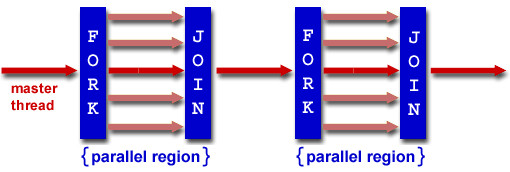
\includegraphics[width=0.5\textwidth]{../images/Schmidt/fork_join.jpg} 
	\caption {Das Fork-Join-Modell zur Parallelisierung einzelner Abschnitte}
	\label{pic:phiForkJoin} 
\end{figure} 
Der Anwendungscode muss für die Parallelisierung mittels OpenMP gegenüber einer seriellen Implementierung nur geringfügig verändert werden. Das Threadingverhalten wird dabei größtenteils durch Compileranweisungen gesteuert. Wie im Codebeispiel \ref{lst:phiOpenMP} zu sehen ist, genügt es ähnlich wie beim Compiler Assisted Offload (siehe Abschnitt \ref{phiCompAssistOffload}) einzelnen Codeabschnitten ein |#pragma| mit der entsprechenden Anweisung voranzustellen. (vgl. \cite{phiOpenmpDoku})
\begin{lstlisting}[language=c, caption={Beispielfunktion mit pragma zur Nebenläufigen Ausführung einer for-Schleife(Quelle: \parencite{phiOpenmpDoku})}, captionpos=b, label=lst:phiOpenMP, frame=single, linewidth=\textwidth, breaklines=true]
double  res[MAX];  int i;
#pragma omp parallel for
for (i=0;i< MAX; i++) {
	res[i] = huge();
}
\end{lstlisting}
Die in Listing \ref{lst:phiOpenMP} gezeigte Anweisung |#pragma omp parallel for| veranlasst den Compiler, einen Code zu erzeugen, der die Schleifendurchläufe nebenläufig ausführt. Die Anzahl der dabei verwendeten Threads lässt sich Umgebungsvariablen und Optionen beim Compileraufruf oder durch den Aufruf von dafür vorgesehenen Bibliotheksfunktionen im Quellcode beeinflussen. (vgl. \cite{phiOpenmpDoku}) Darüber hinaus stellt OpenMP noch eine große Zahl von weiteren Compileranweisungen und Bibliotheksfunktionen bereit. Dies ermöglicht es dem Programmierer zum Beispiel, kritische Abschnitte zu definieren, die nur von maximal einem Thread zur gleichen Zeit bearbeitet werden dürfen. Ein weiteres Beispiel sind Compileranweisungen, mit denen sich bestimmen lässt, ob bestimmte Variablen zwischen den Threads geteilt werden oder ob jeder Thread eine eigene Kopie dieser Variablen erhalten soll. (vgl. \cite{phiOpenmpDoku}) Da die erweiterten Funktionalitäten von OpenMP in diesem Teil der Arbeit nicht erforderlich sind, wird an dieser Stelle auch nicht speziell darauf eingegangen. In einem anderen Teil der Arbeit wird OpenMP näher betrachtet. 

Gegenüber pthread hat die Verwendung von OpenMP geringere Auswirkungen auf die Lesbarkeit und Wartbarkeit eines Programms. Es gibt allerdings Fälle, in denen das Fork-Join-Modell und damit auch OpenMP nicht sinnvoll angewendet werden können. Außerdem werden die zu OpenMP gehörenden |#pragma|-Anweisungen nicht von jedem Compiler unterstützt. Compiler, die diese Anweisungen nicht interpretieren können, sollten diese ignorieren. Dies hat zur Folge, dass der Compiler ein serielles Programm erzeugt, das zwar die gleichen Ergebnisse liefert, dabei aber nicht von Multithreading profitieren kann. (vgl. \cite{phiOpenmpDoku})

\subsection{Intel Threading Building Blocks}
Intel TBB (Threading Building Blocks) ist eine Threadingbibliothek, die Intel für die Programmiersprache C++ entwickelt hat. TBB verfolgt im Gegensatz zu anderen Modellen keinen threadbasierten, sondern einen taskbasierten Ansatz. Dies bedeutet, dass der Programmierer parallelisierbare Operationen nicht mehr in Threads, sondern in einzelne Aufgaben zerlegt, die dann von einem Taskscheduler auf mehrere Threads verteilt werden. Jedes Programm, das mithilfe von TBB zusätzliche Threads erzeugen und verwalten soll, muss zunächst einen Taskscheduler erstellen. Dazu genügt es, ein Objekt des Typs |task_scheduler_init| zu instanziieren. Listing \ref{lst:phiTBBminimalExample} zeigt ein minimales Beispiel, das einen Taskscheduler erstellt und dann endet. (vgl. \cite{intelTBBtutorial})
\begin{lstlisting}[language=c++, caption={Minimalbeispiel zur Verwendung von Intel TBB(Quelle: \parencite{xeonphiBestPractices})}, captionpos=b, label=lst:phiTBBminimalExample, frame=single, linewidth=\textwidth, breaklines=true]
//comment
#include "tbb/task_scheduler_init.h"
#include "tbb/parallel_for.h"
#include "tbb/blocked_range.h"
using namespace tbb;
int main() {
	task_scheduler_init init;
	return 0;
}
\end{lstlisting}
Außerdem ist es möglich, die Aufgaben zu Gruppen zusammenzufassen und Eigenschaften oder Beziehungen für diese festzulegen. Auf diese Weise lassen sich auch komplexe Operationen mit kritischen und atomaren Abschnitten und Barrieren definieren. Der Scheduler verteilt die zu bearbeitenden Aufgaben dann ohne weiteres Zutun des Programmierers unter Beachtung der festgelegten Anforderungen auf möglichst viele Threads. (vgl. \cite{intelTBBtutorial}) Listing \ref{lst:phiTBBfibExample} zeigt beispielhaft, wie die Erstellung und Ausführung neuer Tasks aussehen kann. Es zeigt eine Funktion zur rekursiven Berechnung eines Elements der Fibonacci-Folge. In jedem Rekursionsschritt (falls die Abbruchbedingung nicht erfüllt ist) werden zwei neue Threads gestartet, die die beiden vorherigen Elemente auf die gleiche Art rekursiv berechnen. Wenn beide Threads beendet sind, endet auch die Funktion selbst. 
\begin{lstlisting}[language=c++, caption={Rekursive Funktion mit TBB zur Threadverwaltung(Quelle: \parencite{intelTBBtutorial})}, captionpos=b, label=lst:phiTBBfibExample, frame=single, linewidth=\textwidth, breaklines=true]
{
#include "tbb/task_group.h"

using namespace tbb;

int Fib(int n) {
	if( n<2 ) {
		return n;
	} else {
		int x, y;
		task_group g;
		g.run([&]{x=Fib(n-1);}); // spawn a task
		g.run([&]{y=Fib(n-2);}); // spawn another task
		g.wait();                // wait for both tasks to complete
		return x+y;
	}
}
}
\end{lstlisting}
Wie bei OpenMP ist es auch mit TBB möglich, mit nur geringfügigen Codeänderungen Schleifen nebenläufig auszuführen. Bei TBB geschieht dies allerdings nicht mithilfe von Compileranweisungen, sondern mittels eines in der Bibliothek definierten Templates, das anstelle der |for|-Schleife verwendet wird. Als Beispiel für diese Ersetzung dienen die Listings \ref{lst:phiTBBserialFor} und \ref{lst:phiTBBparallelFor}. Das im zweiten Listing gezeigte Template erwartet als Parameter die Grenzen der Laufvariable und einen Lambdaausdruck mit den in der Schleife auszuführenden Operationen. (vgl. \cite{intelTBBtutorial})
\begin{lstlisting}[language=c++, caption={Funktion mit serieller for-Schleife(Quelle: \parencite{intelTBBtutorial})}, captionpos=b, label=lst:phiTBBserialFor, frame=single, linewidth=\textwidth, breaklines=true]
void SerialApplyFoo( float a[], size_t n ) {
	for( size_t i=0; i!=n; ++i ) {
		Foo(a[i]);
	}
}
\end{lstlisting}
\begin{lstlisting}[language=c++, caption={Funktion mit parallel-for-Template(Quelle: \parencite{intelTBBtutorial})}, captionpos=b, label=lst:phiTBBparallelFor, frame=single, linewidth=\textwidth, breaklines=true]
#include "tbb/tbb.h"

using namespace tbb;

void ParallelApplyFoo( float a[], size_t n ) {
	tbb::parallel_for( size_t(0), n, [&]( size_t i ) {
		Foo(a[i]);
	} );
}
\end{lstlisting}
Im Gegensatz zu OpenMP arbeitet TBB nicht mit |#pragma|-Anweisungen und ist somit nicht auf die Unterstützung des verwendeten Compilers angewiesen. Allerdings existiert TBB derzeit nur für die Programmiersprache C++. Für viele Features werden Lambda-Ausdrücke benötigt, die erst ab dem Sprachstandard C++11 definiert sind. Die Verwendung eines Taskschedulers erzeugt zwar zur Laufzeit einen geringen Overhead, bei hinreichend großen und komplexen Operationen lässt sich mit TBB allerdings trotzdem eine höhere Performance erzielen als mit OpenMP. (vgl. \cite{xeonphiBestPractices})

\section{Intel Math Kernel Library}
Wie die einführenden Kapitel gezeigt haben, lässt sich die Berechnung von künstlichen Neuronalen Netzwerken auf eine Reihe von mathematischen Standardoperationen zurückführen, die auch in anderen wissenschaftlichen Bereichen für numerische Berechnungen eingesetzt werden. Aufgrund dieses Bedarfs existieren für viele Prozessoren und Rechenbeschleuniger Bibliotheken, die diese Operationen sehr effizient und für die jeweilige Zielplattform optimiert implementieren. Intel hat für seine Prozessoren die Bibliothek MKL (Math Kernel Library) entwickelt. MKL stellt unter anderem Funktionen für Matrix- und Vektoroperationen, vektoriesierte Berechnung von mathematischen Funktionen, sowie Generierung von Zufallszahlen bereit. Darüber hinaus unterstützen viele Funktionen der MKL auch die automatische Auslagerung an Coprozessoren wie den in diesem Teil der Arbeit verwendeten Xeon Phi. Intel stellt vorkompilierte Versionen der MKL für die Architekturen IA-32, Intel64, sowie MIC zur Verfügung. Somit kann MKL nicht nur für Offload-Modelle zum Einsatz kommen, sondern auch nativ auf dem Xeon Phi verwendet werden. (vgl. \cite{MKLdevReference})

\subsection{Basic Linear Algebra Subprograms}
Basic Linear Algebra Subprograms (BLAS) ist ein De-facto-Standard für Bibliotheken, die Funktionen zur Berechnung von Vektor-Vektor-Operationen, Matrix-Vektor-Operationen und Matrix-Matrix-Operationen bereitstellen. Für diese Bibliotheken gibt es viele hochperformante Implementierungen, die von Hardwareherstellern speziell für deren Prozessoren optimiert wurden. Diese sind untereinander relativ leicht austauschbar, da die darin definierten Funktionen einheitlichen Namenskonventionen folgen und identische Parameterlisten besitzen. Auch in MKL ist eine BLAS-Bibliothek enthalten. (vgl. \cite{MKLdevReference})

Als Beispiel für eine BLAS-Funktion sei an dieser Stelle die Funktionsdeklaration von |cblas_sgemm| in Listing \ref{lst:mklBlasGemm} genannt. Die Funktion beschreibt eine Operation der Form \(C := alpha*op(A)*op(B) + beta*C\), wobei \(A\), \(B\) und \(C\) Matrizen sind. \(alpha\) und \(beta\) sind in dieser Gleichung Skalare. Der Operator \(op\) kann gibt an, dies die Matrix in dessen Argument transponiert werden kann. (vgl. \cite{MKLdevReference})
\begin{lstlisting}[language=c++, caption={Deklaration einer BLAS-Funktion zur Matrix-Matrix-Multiplikation(Quelle: \parencite{MKLdevReference})}, captionpos=b, label=lst:mklBlasGemm, frame=single, linewidth=\textwidth, breaklines=true]
void cblas_sgemm (const CBLAS_LAYOUT Layout, const CBLAS_TRANSPOSE transa, const CBLAS_TRANSPOSE transb, const MKL_INT m, const MKL_INT n, const MKL_INT k, const float alpha, const float *a, const MKL_INT lda, const float *b, const MKL_INT ldb, const float beta, float *c, const MKL_INT ldc);
\end{lstlisting}
Nachfolgend werden die Funktionsparameter aus Listing \ref{lst:mklBlasGemm} näher erläutert. 
\begin{description}
\item{Layout:} enum-Wert, der angibt, ob das Array mit den Zahlenwerten der Ergebnismatrix column-major oder row-major zu lesen ist. 
\item{transa: } enum-Wert, der angibt, ob \(A\) vor der Matrix-Matrix-Multiplikation transponiert werden soll. Das übergebene Array bleibt dabei unverändert, der Funktion wird nur mitgeteilt, dass das Array entgegen der in |Layout| angegebenen Leserichtung zu lesen ist. 
\item{transb: } wie |transa|, bezieht sich aber auf Matrix \(B\). 
\item{m: } Anzahl der Zeilen in Matrix \(C\)
\item{n: } Anzahl der Spalten in Matrix \(C\)
\item{k: } Anzahl der Spalten in Matrix \(op(A)\) bzw. der Zeilen in Matrix \(op(B)\)
\item{alpha: } Wert des Skalars \(alpha\)
\item{a: } Pointer auf ein Array mit den Werten der Matrix \(A\)
\item{lda: } Leading Dimension der Matrix \(A\). Dieser Parameter ist nützlich, wenn das Array |a| eine größere Matrix enthält, von der nur ein Teil betrachtet werden soll. Je nach Leserichtung der Matrix gibt dieser Wert den Abstand zwischen dem ersten Element der ersten Zeile/Spalte und dem ersten Element der zweiten Zeile/Spalte an. 
\item{b: } Pointer auf ein Array mit den Werten der Matrix \(B\)
\item{ldb: } Wie |lda|, bezieht sich aber auf Matrix \(B\)
\item{beta: } Wert des Skalars \(beta\)
\item{c: } Pointer auf ein Array mit den Werten der Matrix \(C\)
\item{ldc: } Wie |lda|, bezieht sich aber auf Matrix \(C\)
\end{description}
Wie das Beispiel zeigt, müssen die Matrizen nicht in Objekte gekapselt werden. Stattdessen benötigen die BLAS-Funktionen Arrays mit Zahlenwerten und zusätzliche Informationen, wie diese als Matrizen zu interpretieren sind. Für diese Interpretation wird dem Programmierer ein großer Spielraum eingeräumt; es sind alle Kombinationen von Leserichtungen erlaubt und für jede Matrix lässt sich eine Leading Dimension angeben. Eine Ausnutzung dieser Flexibilität ermöglicht es, aufwändiges Kopieren und Umstrukturieren der zu verarbeitenden Daten zwischen den tatsächlichen Rechenoperationen weitgehend zu vermeiden. (vgl. \cite{MKLdevReference})

\subsection{Vector Mathematical Functions}
Mithilfe der BLAS-Funktionen lassen sich Aufgaben aus dem Gebiet der linearen Algebra mit geringem Programmieraufwand auch für größere Datenmengen performant berechnen. Allerdings müssen in neuronalen Netzwerken auch nichtlineare Funktionen für grüßere Datenmengen berechnet werden. Notwendig ist dies speziell bei der Aktivierungsfunktion und der Ermittlung der Kosten. Für die vektorisierte Berechnung von nichtlinearen Operationen stellt MKL zusätzliche Funktionen bereit. Ein Beispiel liefert die Funktion |vsTanh( n, a, y );| Diese berechnet den Tangens Hyperbolicus von allen Elementen des Vektors |a| und speichert die Ergebnisse in Vektor |y|. Aus Sicht des Programmierers sind |a| und |y| Pointer auf Arrays der Größe |n|. Im Gegensatz zu BLAS-Routinen wird die Ausführung dieser Funktionen nicht auf mehrere CPU-Kerne verteilt. Dennoch werden die Berechnungen innerhalb eines Kerns unter Verwendung spezieller Hardware für SIMD-Berechnungen(Single Instruction Multiple Data) parallelisiert. (vgl. \cite{MKLdevReference})

\subsection{Statistical Functions}
Entscheidend für die Genauigkeit, die ein CNN erreichen kann, ist die Verteilung der Gewichte im Initialzustand. Idealerweise sollte der Durchschnitt aller Gewichte bei \(0\) liegen, wobei die Gewichte mit geringer Varianz verteilt sein sollten, sodass sich die Featuremaps innerhalb eines Layers unterschiedlich entwickeln können. (vgl. \cite{neuralNetworksAndDeepLearning})

Zur Generierung von Zufallszahlen, mit denen die Gewichte initialisiert werden können, stellt Intel in MKL eine Reihe von Zufallszahlengeneratoren zur Verfügung. (vgl. \cite{MKLdevReference}) Die Anforderungen an die Geschwindigkeit sind bei der Initialisierung der Gewichte niedriger als bei der späteren Anpassung, da die Initialisierung nur einmalig zum Start des Programms erfolgt. Entscheidend für die Genauigkeit des Netzwerks nach dem Training ist, dass die Verteilung der Anfangsgewichte den oben genannten Anforderungen entspricht. Für die in diesem Teil zu erstellende Implementierung wird eine Gaußverteilung gewählt. 


\section{Grundlegende Überlegungen}
Der eigentlichen Implementierung des Trainingsprogramms für das CNN gehen einige konzeptionelle Überlegungen voraus. In diesem Abschnitt werden einige grundlegende Designentscheidungen festgehalten, die Einfluss auf die Programmarchitektur und damit indirekt auf die Effizienz und Änderbarkeit des entstehenden Programms haben werden. 

\subsection{Parallelisierung}
Das Trainieren des Netzwerks ist im Wesentlichen ein iterativer Prozess, der seriell abgearbeitet werden muss. Nebenläufig abarbeiten lässt sich nicht der gesamte Prozess, sondern nur einzelne Operationen innerhalb des Prozesses. Konkret bedeutet das zum Beispiel, dass zunächst die Fehler der Gewichte berechnet werden müssen, bevor auf Basis dieser Fehler die Anpassung der Gewichte berechnet werden kann. Beide Operationen für sich können durch Nebenläufigkeit beschleunigt werden, allerdings darf nicht mit der Bearbeitung des zweiten Schritts begonnen werden, bevor der erste Schritt abgeschlossen ist. Für diese Arbeit bedeutet dies, dass das Fork-Join-Modell zur Parallelisierung am besten geeignet ist. Viele Routinen aus der MKL-Bibliothek sind bereits so implementiert, dass sie automatisch nebenläufig ausgeführt und bei Bedarf ausgelagert werden. Für parallelisierbaren Anwendungscode wird OpenMP verwendet, da diese Bibliothek am einfachsten zu verwenden ist. Es darf angenommen werden, dass die dabei entstehenden Threads nicht auf geteilte Variablen schreiben und daher keine zusätzliche Synchronisierung notwendig ist. Somit ließe sich durch die Verwendung von TBB im Anwendungscode gegenüber OpenMP wohl kein nennenswerter Performancegewinn erzielen. 

\subsection{Programmiersprache}
Um eine möglichst gute Performance zu erzielen, muss eine Sprache verwendet werden, die zu Maschinencode kompiliert werden kann. Andernfalls müsste das Programm zur Laufzeit interpretiert werden, was zusätzlichen Aufwand verursachen würde. Die verwendeten Bibliotheken OpenMP, sowie MKL unterstützen die Sprachen C, C++ und Fortran. Die Implementierung des Programms erfolgt größtenteils in C, eine Ausnahme stellt der Code dar, der die Eingabedaten und Labels des MNIST-Datensatzes von der Festplatte einliest. Dieser Code wird mit geringen Veränderungen von der seriellen Implementierung übernommen und benötigt Funktionen, die in C++-Bibliotheken definiert sind und in C nicht direkt verwendet werden können. Die Deklarationen der in C++ geschriebenen und von C-Code aufgerufenen Funktionen werden mit dem Schlüsselwort |extern "C"| versehen, sodass sie anschließend vom Linker gebunden werden können. 

Die Entscheidung für die Programmiersprache C ist mit den bevorzugten Paradigmen der Programmiersprachen C und C++ zu begründen. C ist eine strukturierte Programmiersprache, während C++ objektorierte Ansätze verfolgt. Zu diesen Ansätzen gehören auch Vererbungshierarchien und Polymorphie. Diese Ansätze erleichtern dem Programmierer zwar die Arbeit, allerdings macht die Verwendung dieser Ansätze dynamische Typbindung erforderlich. Das bedeutet, dass beim Aufruf von Funktionen, die in einer Vererbungshierarchie mehrfach implementiert wurden, zur Laufzeit entschieden wird welche Implementierung letztendlich aufgerufen wird. Die Verwendung von dynamisch gebundenen Funktionen macht den Code langsamer und wird aus diesem Grund bewusst vermieden. Auch bestimmte Design Patterns, die auf mehrfacher Delegation von Funktionsaufrufen zwischen mehreren ähnlichen Objekten basieren wird bewusst abgesehen. 

Tatsächlich soll der serielle Teil des zu erstellenden Programms möglichst schnell nacheinander nebenläufige Funktionen für die eigentlichen Rechenoperationen aufrufen. Der Code, der zwischen den Aufrufen steht, sollte möglichst kurz und möglichst sequentiell sein, also keine unnötigen Verzweigungen enthalten. 

\subsection{Codegenerierung} \label{xeonphi:codegen}
Zu den Anforderungen gehört auch eine Änderbarkeit des verwendeten Netzwerkmodells und der Programmkonfiguration. 
Eine gute Änderbarkeit ist dann gegeben, wenn das Netzwerkmodell an nur einer Stelle geändert werden muss, um das Programm anzupassen. Die gebräuchlichste Möglichkeit, diese Änderbarkeit zu erreichen, ist die Definition einer Liste von Objekten einer gemeinsamen Basisklasse, die die einzelnen Netzwerkschichten repräsentieren. Zur Veränderung des Netzwerkmodells müsste nur die Initialisierung dieser Liste geändert werden. Bei der Simulation des Netzwerkes könnte dann auf verschiedene Implementierungen von Methoden zurückgegriffen werden, die für die verschiedenen Layertypen definiert sind. 
Dieser Ansatz steht allerdings in Widerspruch zur Entscheidung, auf dynamische Typbindung und somit Vererbung zu verzichten. Um eine objektorientierte Beschreibung des Netzwerks zu ermöglichen und gleichzeitig alle Strukturen und Methoden statisch zu binden, wird die Implementierung des CNNs für den Xeon Phi in zwei Programme aufgeteilt: 

Der erste Teil ist ein Python-Skript, das ähnlich wie bei Tensorflow ein neuronales Netzwerk anhand seiner Schichten und deren Eigenschaften beschreibt. Außerdem werden in diesem Skript einige Einstellungen festgelegt, die das Verhalten des Programms während des Trainings festlegen. 

Der zweite Teil ist das eigentliche Programm zum Trainieren des Netzwerks. Dieses ist in C geschrieben und benötigt an mehreren Stellen Informationen über den Aufbau des Netzes und Details über einzelne Schichten. An diesen Stellen wird C-Code generiert, der alle notwendigen Informationen bereits enthält. Teilweise können dadurch Berechnungen schon vor der Übersetzung durchgeführt und deren Ergebnisse als Konstanten in den Code eingefügt werden. Die Verwendung von Konstanten anstatt zur Laufzeit berechneter Variablen ermöglicht es dem Compiler, den ausführbaren Code zusätzlich zu optimieren und Speicherzugriffe zu reduzieren. 

Zur Codegenerierung wird das Python-Tool |cog| verwendet. Dieses Tool kann Textdateien nach speziell formatierten Zeilen durchsuchen. Diese Zeilen markieren den Anfang und das Ende eines Python-Codes. Dieser Python-Code erzeugt eine Ausgabe, die zwischen dem Ende des markierten Abschnitts und einer dritten Markierung eingefügt wird. Die Markierungen sind so gewählt, dass der Python-Code aus Sicht des C-Programms wie ein Kommentar erscheint. (vgl. \cite{COGdocumentation})

Zum Ändern des Netzwerkmodells oder der Konfiguration genügt es, das entsprechende Python-Skript anzupassen und anschließend |cog| mit einigen Quellcodedateien des C-Codes aufzurufen. Der dabei entstehende Code kann anschließend in ein lauffähiges Programm übersetzt werden, das der zuvor festgelegten Konfiguration entspricht. 

\subsection{Datenorganisation}
Bei der seriellen Implementierung werden zur Laufzeit mehrmals pro Trainingsdurchlauf temporäre Matrizen erzeugt, für die jeweils Speicher alliziert werden muss. Die Speicherallozierung ist ein zeitraubender Prozess, daher wird in diesem Teil der Arbeit schon früh ein Konzept zur Speicherverwaltung erarbeitet. 

Die für temporäre Zwischenergebnisse wird in der Initialisierungsphase des Programms ein zusammenhängender Speicherbereich reserviert und für den gesamten Rest der Laufdauer im Speicher gehalten. Funktionen, die temporäre Zwischenergebnisse ablegen müssen, können diesen Speicherbereich verwenden. Es ist allerdings sicherzustellen, dass keine Ergebnisse überschrieben werden, die später noch benötigt werden. Die Größe dieses Speichers hängt vom verwendeten Netzwerkmodell und der Batchsize ab, aus diesem Grund wird der Code zur Speicherreservierung generiert. 

Beim Durchlaufen des Netzwerks (sowohl vorwärts als auch rückwärts) werden in jedem Layer Aktivierungen bzw. Fehler berechnet, die vom nachfolgenden bzw. vorhergehenden Layer als Eingaben benötigt werden. Diese Aktivierungen sollten nicht von einem Layer zum nächsten kopiert werden, denn dies wäre eine unnötige Operation. Stattdessen sollen beide Layer je einen Pointer besitzen, der auf die gleiche Speicheradresse zeigt. Diese Pointer können ohne weitere Verarbeitung zum Aufruf von MKL-Funktionen verwendet werden. Da beide Pointer auf einen gemeinsamen Speicherbereich zeigen, stellt sich die Frage, welcher Layer für diesen Speicherbereich verantwortlich ist, also diesen Initialisieren soll. Außerdem müsste dieser Layer seinen Nachbarn über die Speicheradresse informieren, was erforderlich machen würde, dass die Layer Kenntnis voneinander besitzen. Um dies zu vermeiden, wird der Speicher für sämtliche Aktivierungen als ein zusammenhhängender Speicher reserviert und die Startadresse in einer Struktur festgehalten, die das gesamte Netzwerk repräsentiert. Diese Struktur beinhaltet weitere Strukturen, die die einzelnen Layer repräsentieren. Darin finden sich Pointerk, die in den reservierten Speicherbereich hineinzeigen. Sowohl die Definition der Netzwerkstruktur, als auch die Funktion zur Initialisierung müssen mit |cog| generiert werden, das die Abfolge der Layer, deren Größenangaben und die daraus ermittelbare Gesamtgröße des Aktivierungsfeldes vom Aufbau Netzwerkmodells abhängen. Jeder Aktivierung lässt sich genau ein Fehler zuordnen, der in der Backpropagation ermittelt werden kann. Daher kann in der Netzwerkstruktur ein zweiter Speicherbereich mit identischer Größe erzeugt werden, für den die Layer zusätzliche Pointer mit identischen Offsets innerhalb des Feldes erhalten. 

Ähnlich wie die Aktivierungen werden auch die Gewichte und Biases aller Layer des Netzwerks in einem zusammenhängenden Array gespeichert. Wie zuvor wird auch ein zweites Array mit gleicher Größe und Einteilung für die Fehler der Aktivierungen angelegt. Obwohl für die Gewichte eindeutig feststellbar ist, zu welchen Layern sie gehören, ist diese Einteilung von Vorteil: Bei der Durchführung des Gradient Descent müssen die berechneten Fehler der Gewichte skaliert und von den eigentlichen Gewichten subtrahiert werden. Wenn diese jeweils in einem großen Array statt in vielen kleinen Feldern stehen, dann kann die Hardware zur Vektorisierung für den Gradient Descent besser eingesetzt werden. 

Die Trainings- und Testdaten werden während der Initialisierung vollständig geladen und während der gesamten Laufzeit im Speicher gehalten. Um unnötige Rechenschritte einzusparen, sollen die Eingabedaten nicht vor der Vorwärtspropagierung in das Aktivierungsfeld kopiert werden. Stattdessen soll der erste Layer einen Pointer erhalten, der auf die Eingabedaten verweist. Für die Vorwärts- und Rückwärtsberechnung innerhalb eines Layers werden aus diesm Grund je zwei Funktionen geschrieben. Eine der beiden Funktionen beschreibt das normale Verhalten des Layers, die andere den Sonderfall, dass es sich um den ersten Layer handelt und ein zusätzlich übergebener Pointer für die Eingabedaten verwendet werden muss. Auch wenn, dadurch die Codesize und der Wartungsaufwand wegen redundantem Code steigt, lohnt sich diese Art der Implementierung: Welcher Layer der erste im Netzwerk ist, lässt sich schon im Schritt der Codegenerierung bestimmen. In jedem Trainingsschritt für jeden Layer und die Berechnung in beide Richtungen mithilfe von Verzweigungen die zu verwendende Eingabeadresse zu bestimmen, wäre ein signifikanter Mehraufwand zur Laufzeit des Programms. 

\subsection{Convolution und Pooling} \label{xeonphi:convnpool}
Im vorherigen Abschnitt wurde bereits erwähnt, dass jeweils zwei benachbarte Layer gemeinsame Speicherbereiche zum Austausch von Aktivierungen und deren Fehlern verwenden. Damit die darin enthaltenen Ergebnisse richtig interpretiert werden können, benötigen diese Layer aber zusätzliche Informationen. Grundsätzlich lässt eine Anordnung von Aktivierungen im Ausgang einer Schicht als vierdimensionaler Tensor verstehen. Die Größe des Tensors ist aufgrund des Netzwerkmodells bekannt, für die Anordnung der Zahlenwerte im Speicher wird an dieser Stelle eine Konvention festgelegt. Die Ablage der Aktivierungswerte erfolgt im Normalfall nach dem Schema BYXF. Die einzelnen Buchstaben lassen sich ähnlich wie Ziffern in einem Zahlensystem interpretieren interpretieren: Werden zwei aufeinanderfolgende Features(F) an der gleichen Position(Y-X) innerhalb des gleichen Elements einer Minibatch(B) betrachtet, dann stehen die dazugehörigen Werte direkt hintereinander im Speicher. Eine Position innerhalb eines vierdimensionalen Tensors kann somit auch als eine Zahl des Schemas BYXF interpretiert werden; diese wiederrum lässt sich als Offset innerhalb eines eindimensionalen Arrays bzw. zusammenhängenden Speicherbereichs verstehen, das alle Aktivierungen des Tensors enthält. 

Es gibt allerdings eine Ausnahme: Nach einem Convolutional Layer werden die Daten in einer anderen Reihenfolge abgelegt. Grund dafür ist eine Optimierung der Faltungsoperation, die Auswirkungen auf die Struktur des Ergebnisses hat. Pooling Layer sind in dieser Implementierung darauf ausgelegt, sowohl die normale Reihenfolge nach dem Schema BYXF, als auch die Ausgabe eines Convolutional Layers als Eingabe verarbeiten zu können. Für alle anderen Layertypen gilt dies nicht, aus diesem Grund muss auf jeden Convolutional Layer ein Pooling Layer folgen. Da dies bei CNNs normalerweise sowieso der Fall ist, stellt dies in den meisten Fällen keine Einschränkung dar. Sollte es tatsächlich erforderlich sein, dass eine Faltungsoperation ohne nachfolgendes Pooling durchgeführt wird, so muss als Workaround ein Pooling Layer mit der Filtergröße 1x1 in das Netzwerkmodell eingefügt werden. Tatsächlich findet dann keine Reduktion der Datenmenge statt, aber die zu verarbeitenden Daten werden in eine Reihenfolge gebracht, die von allen nachfolgenden Layern verarbeitet werden kann. Einzelheiten zur Implementierung der Faltungsoperation und des Poolingalgorithmus befinden sich in den entsprechenden Unterkapiteln in diesem Teil der Arbeit. 

\subsection{Buildsystem}
Das zu erstellende Programm soll nicht nur auf dem Rechner des Studenten, sondern auch auf dem Server der DHBW und auf weiteren Rechnern übersetzt werden können. Dies macht das ein Buildsystem erforderlich, das die Übersetzung sowohl unter Windows, als auch unter Linux und unixbasierten Systemen ermöglicht. 

Der Build des ausführbaren Programms erfolgt in mehreren Schritten: 
\begin{description}
\item{Konfiguration: } Zunächst kann der Nutzer durch Modifikation der dafür vorgesehenen Pythonskripte ein Netzwerkmodell, sowie eine Konfiguration festlegen. 
\item{Codegenerierung: } Nach einer Konfigurationsänderung muss ein Teil des C-Programms neu generiert werden. Dazu wird das Python-Tool |cog| benötigt. (vgl. \cite{COGdocumentation}) Mit dem Befehl |cog -r @COG_filelist.txt| wird die Codegenerierung gestartet. Die ersten beiten Schritte können auch übersprungen werden, in diesem Fall wird die Konfiguration zum Zeitpunkt der Abgabe dieser Arbeit verwendet. 
\item{Build: } Nach der Codegenerierung kann das Programm wie jedes andere C-Programm durch Kompilierung aller Codedateien und anschließendes Linken übersetzt werden. Der ICC-Compiler muss unter Windows anders aufgerufen werden als unter Linux, daher unterscheiden sich die Buildprozesse geringfügig. Für die Übersetzung auf Linuxsystemen existiert eine Makefile zur Automatisierung des Buildvorgangs. Wenn GNU make auf dem System installiert ist, dann lässt sich der Build mit |make all| starten. Um zwischen den Usage Modellen Native und Offload wechseln zu können, wird am Anfang der Makefile eine Variable Namens |MK_PHI_USAGE_MODEL| definiert. Eine Änderung des Wertes dieser Variable führt zu einem Build mit dem jeweiligen Nutzungsmodell. Für Windows-Systeme gibt es ein alternatives Buildsystem auf Basis von SCons. 
\item{Ausführung: } Beim Build wird die ausführbare Datei |build/program| erzeugt. Diese Datei beinhaltet das CNN-Trainingsprogramm und kann mit |./build/program| gestartet werden. Alternativ kann mit |make execute| das Programm übersetzt und nach dem erfolgreichen Build automatisch gestartet werden. Die Ausgaben des Programms selbst, sowie eines Tools zur Messung der Ausführungsdauer werden in die Datei |report.txt| geschrieben. 
\end{description}

\section{Skript zur Netzwerkbeschreibung}
Wie in Abschnitt \ref{xeonphi:codegen} bereits erläutert wurde, wird in dieser Implementierung zusätzlich zum eigentlichen C-Programm ein Pythonskript erstellt, das zur Modellierung des Netzwerkes dient. In diesem Abschnitt wird dieses Skript näher beschrieben. 

\subsection{Klasseneinteilung}
\begin{figure}
	\centering 
	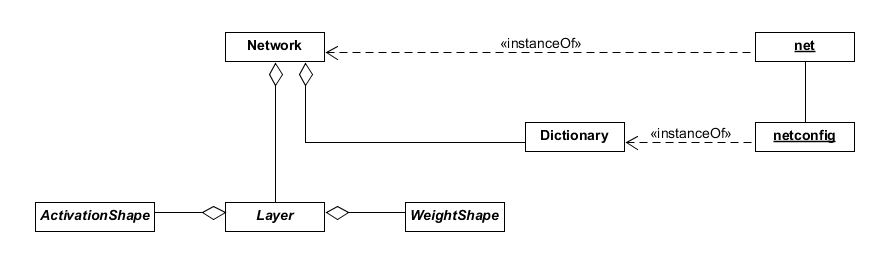
\includegraphics[width=\textwidth]{../images/Schmidt/cd_netdesc.jpg} 
	\caption {Klassendiagramm des Skripts zur Netzwerkbeschreibung}
	\label{pic:cd_Netdesc} 
\end{figure} 
Das Klassendiagramm aus Abbildung \ref{pic:cd_Netdesc} soll zunächst einen groben Überblick  über den Aufbau des Netzwerkmodells verschaffen. Repräsentiert wird ein CNN durch die Klasse |Network|. Objekte dieser Klasse besitzen je ein Dictionary zur Festlegung der Konfiguration und eine Liste von Objekten des abstrakten Typs |Layer|. Jeder |Layer| besitzt zwei Referenzen auf Objekte des Typs |ActivationShape|, wobei eine für die Aktivierungen am Eingang und eine für die Aktivierungen am Ausgang steht. Darüber hinaus besitzt jeder Layer Ein Objekt des abstrakten Typs |WeightShape|. |ActivationShape| beschreibt einen Tensor mit Aktivierungen, und beschreibt die Schnittstelle zwischen zwei Schichten bzw. zwischen einer Schicht und dem Ein- oder Ausgang des Netzes. 

In der Datei |src/NetworkDescriptor/NetInstance.py| wird mit dem Opjekt |net| eine Instanz der Klasse Network erstellt. Zusätzlich wird aus der Datei |src/NetworkDescriptor/NetConfig.py| ein Dictionary mit den Konfigurationsdaten importiert. Alle Pythonskripte, die für die Codegenerierung verantwortlich sind, importieren das beschriebene Objekt |net| und verwenden die darin enthaltenen Daten, d.h. durch eine Änderung der Definition von |net| und anschließende Codegenerierung lässt sich das Verhalten des C-Programms beeinflussen. 

\subsection{Netzwerk}
Zur Erstellung eines Objekts der Klasse |Network| wird eine |ActivationShape| zur Beschreibung des Tensors für die Eingangsdaten, sowie ein Dictionary mit der Konfiguration benötigt. 

Ist das Netzwerk einmal erstellt, lassen sich der Reihe nach Schichten zum Netzwerk hinzufügen. Dazu steht für jede instanziierbare Unterklasse von Layer eine Methode zur Verfügung. Diese Methoden rufen die jeweiligen Konstruktoren der entsprechenden Typen auf und übergeben die Argumente, die sie selbst erhalten haben, sowie die |ActivationShape| für die Ausgaben der letzten Schicht des Netzwerks. Mithilfe dieser Informationen generiert der Konstruktor eine |ActivationShape|, die den Ausgangstensor einer Netzwerkschicht mit den durch die Parameter bestimmten Eigenschaften beschreibt. Anschließend wird der neue |Layer| in die Liste der Netzwerkschichten aufgenommen, wobei die gleichzeitig erstellte |ActivationShape| zur letzten des Netzwerks wird und somit dem nächsten hizuzufügenden Layer als Eingangstensor übergeben werden kann. 

Nachdem alle Schichten hinzugefügt wurden, muss die Methode |generate| aufgerufen werden. In dieser Methode werden anhand der im Netzwerkmodell enthaltenen Informationen über die Schichten und deren Schnittstellen, zusätzliche Informationen berechnet, die bei der Generierung des C-Codes benötigt werden. Dazu gehören Beispielsweise die Startpositionen für die Tensoren innerhalb des Feldes mit den Aktivierungen bzw. deren Fehlern. Diese Startpositionen entsprechen jeweils der Startposition des vorherigen Layers, erhöht um dessen Größe. Optional kann dieser Betrag zusätzlich auf das nächste Vielfache des Konfigurationsparameters |CONFIG_ARRAY_ALIGNMENT| erhöht werden. Bei der Speicherallozierung der Felder zur Laufzeit des C-Programms wird ebenfalls mit dem gleichen Alignment gearbeitet. Somit ist Sichergestellt, dass alle Adressen, die zur Laufzeit als Beginn von Matrizen verwendet werden, auf dieses Alignment eingestellt sind. Laut der Dokumentation von MKL können die Bibliothekensfunktionen effizienter arbeiten, wenn sie ein Alignment von 256 Byte aufweisen. (vgl. \cite{MKLdevReference}) 

\subsection{Schnittstellen zwischen Schichten}
\begin{figure}
	\centering 
	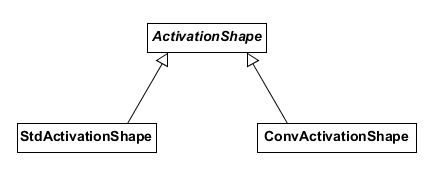
\includegraphics[width=\textwidth]{../images/Schmidt/cd_netdesc_actshapes.jpg} 
	\caption {Unterklassen von ActivationShape}
	\label{pic:cd_Netdesc_actshapes} 
\end{figure} 
Wie im Abschnitt \ref{xeonphi:convnpool} bereits vorweggenommen wurde, erzeugt ein Convolutional Layer eine Ausgabe, deren Größe und Reihenfolge sich von denen der anderen Schichttypen unterscheidet. Diese Besonderheit muss im Netzwerkmodell berücksichtigt werden. Aus diesem Grund besitzt die abstrakte Klasse |ActivationShape| zwei instanziierbare Unterklassen. (siehe Abbildung \ref{pic:cd_Netdesc_actshapes}) Die Unterklasse |StdActivationShape| beschreibt einen Aktivierungstensor des Formats BYXF, wie er von den meisten Layertypen als Eingang verwendet und für den Ausgang erzeugt wird. |ConvActivationShape| beschreibt ein spezielles Format, das nur an der Schnittstelle von einem Convolutional Layer zu einem Pooling Layer verwendet werden kann. 

Beide Unterklassen implementieren mehrere in der Oberklasse definierte get-Accessoren. Damit lassen sich die Dimensionen des Tensors in die Richtungen B, Y, X und F, sowie der tatsächliche Speicherbedarf für alle enthaltenen Werte abfragen. Außerdem sind get-Accessoren enthalten, mit denen sich die Speicherposition eines Aktivierungswertes innerhalb des Tensors anhand seiner Koordinaten ermitteln lässt. 

\subsection{Gewichtsspeicherung}
\begin{figure}
	\centering 
	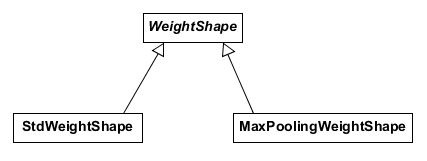
\includegraphics[width=\textwidth]{../images/Schmidt/cd_netdesc_weightshapes.jpg} 
	\caption {Unterklassen von WeightShape}
	\label{pic:cd_Netdesc_weightshapes} 
\end{figure} 
Auch die Klasse |WeightShape| ist abstrakt und besitzt zwei instanziierbare Unterklassen. 

\subsection{Layertypen}

\subsection{Netzwerkkonfiguration}



\section{Programm zur Netzwerksimulation}

\subsection{Moduleinteilung}

\subsection{Netzwerkmodell}

\subsection{Netzwerkinitialisierung}

\subsection{Hilfsfunktionen}

\subsection{Verhaltensbeschreibung der Layer}

\subsection{Datenfluss beim Fully Connected Layer}

\subsection{Organisation der Faltungsoperation}

\subsection{Implementierung des Poolings}

\subsection{Programmfluss}



\section{Anpassung der Netzwerkkonfiguration}

\subsection{Startgewichte}

\subsection{Reduzierung der Lernrate}

\subsection{Fehlerreduktion beim Convolution Layer}


\section{Vergleich mit Tensorflow}



\end{document}